% Options for packages loaded elsewhere
\PassOptionsToPackage{unicode}{hyperref}
\PassOptionsToPackage{hyphens}{url}
%
\documentclass[
]{article}
\usepackage{amsmath,amssymb}
\usepackage{lmodern}
\usepackage{ifxetex,ifluatex}
\ifnum 0\ifxetex 1\fi\ifluatex 1\fi=0 % if pdftex
  \usepackage[T1]{fontenc}
  \usepackage[utf8]{inputenc}
  \usepackage{textcomp} % provide euro and other symbols
\else % if luatex or xetex
  \usepackage{unicode-math}
  \defaultfontfeatures{Scale=MatchLowercase}
  \defaultfontfeatures[\rmfamily]{Ligatures=TeX,Scale=1}
\fi
% Use upquote if available, for straight quotes in verbatim environments
\IfFileExists{upquote.sty}{\usepackage{upquote}}{}
\IfFileExists{microtype.sty}{% use microtype if available
  \usepackage[]{microtype}
  \UseMicrotypeSet[protrusion]{basicmath} % disable protrusion for tt fonts
}{}
\makeatletter
\@ifundefined{KOMAClassName}{% if non-KOMA class
  \IfFileExists{parskip.sty}{%
    \usepackage{parskip}
  }{% else
    \setlength{\parindent}{0pt}
    \setlength{\parskip}{6pt plus 2pt minus 1pt}}
}{% if KOMA class
  \KOMAoptions{parskip=half}}
\makeatother
\usepackage{xcolor}
\IfFileExists{xurl.sty}{\usepackage{xurl}}{} % add URL line breaks if available
\IfFileExists{bookmark.sty}{\usepackage{bookmark}}{\usepackage{hyperref}}
\hypersetup{
  pdftitle={The Causal Impact of Romneycare on Massachusetts' Mortality Rate using Synthetic Control},
  pdfauthor={Elle Boodsakorn, Parker Gauthier, Amal Kadri, Alice Kemp and Austin Longoria},
  hidelinks,
  pdfcreator={LaTeX via pandoc}}
\urlstyle{same} % disable monospaced font for URLs
\usepackage[margin=1in]{geometry}
\usepackage{graphicx}
\makeatletter
\def\maxwidth{\ifdim\Gin@nat@width>\linewidth\linewidth\else\Gin@nat@width\fi}
\def\maxheight{\ifdim\Gin@nat@height>\textheight\textheight\else\Gin@nat@height\fi}
\makeatother
% Scale images if necessary, so that they will not overflow the page
% margins by default, and it is still possible to overwrite the defaults
% using explicit options in \includegraphics[width, height, ...]{}
\setkeys{Gin}{width=\maxwidth,height=\maxheight,keepaspectratio}
% Set default figure placement to htbp
\makeatletter
\def\fps@figure{htbp}
\makeatother
\setlength{\emergencystretch}{3em} % prevent overfull lines
\providecommand{\tightlist}{%
  \setlength{\itemsep}{0pt}\setlength{\parskip}{0pt}}
\setcounter{secnumdepth}{-\maxdimen} % remove section numbering
\usepackage{booktabs}
\usepackage{longtable}
\usepackage{array}
\usepackage{tabu}
\ifluatex
  \usepackage{selnolig}  % disable illegal ligatures
\fi

\title{The Causal Impact of Romneycare on Massachusetts' Mortality Rate
using Synthetic Control}
\author{Elle Boodsakorn, Parker Gauthier, Amal Kadri, Alice Kemp and
Austin Longoria}
\date{University of Texas at Austin - ECO395M - Spring 2022}

\begin{document}
\maketitle

\newline
\newline

\hypertarget{abstract}{%
\section{Abstract}\label{abstract}}

We utilize the panel dataset from Center for Disease Control (CDC) to
investigate the effect of Romneycare on mortality rates. Our analysis
uses Synthetic Control to find the optimal weights for each state that
closely resembles Massachusetts. We present these weights as well as our
model prediction of lower mortality rates post 2006, when Romneycare was
passed. Although Massachusetts did not trend similarly to other states
chosen by Synthetic Control prior to the passage of Romneycare in 2006,
our model predicts a decline in mortality rate of .867 which matches the
actual outcome almost exactly. The results of our Synthetic Control
estimates confirm the conclusion of Sommers, Long, and Baicker. \newpage

\hypertarget{introduction}{%
\section{1. Introduction}\label{introduction}}

Access to healthcare through affordable health insurance remains one of
the most divisive policy debates in the United States, with critics of a
privatized system arguing in favor of a widespread, easily accessible
option targeted at low income households to increase the quality and
quantity of health care. However, some supporters of private insurance
argue against such a system, stating that insurance provided by the
federal government unfairly burdens taxpayers, many of whom opt for
private coverage through their employers. Before the groundbreaking
introduction of the Affordable Care Act in 2008, better known as
``Obamacare'', the state of Massachusetts passed its own state-provided
health insurance program signed into law by Senator Mitt Romney in 2006.
The program, dubbed ``Romneycare'' and the first of its kind in the
U.S., provided free and heavily subsidized health insurance to the
lowest income resident of the state, and mandated that nearly all
residents obtain a minimal level of coverage. To aid in the provision of
coverage to higher earners, the law also required every employer in the
state with over ten full-time employees to provide a health insurance
plan to workers. Before the program was heavily rolled back in favor of
Obamacare in 2012, over 97\% of Massachusetts residents had health
insurance coverage. Many studies have investigated the effects of
Romneycare and Obamacare on statistics such as health coverage,
insurance utilization, and health care pricing, however, few have
attempted to isolate the causal effect of mandated affordable health
coverage on mortality rates. One of the reasons why this effect can be
difficult to identify is due to the distribution of health care in the
U.S. - as insurance is not randomly assigned to individuals but normally
obtained through employers, low income individuals tend to have minimal
coverage, if at all and sub-optimal quality of care. As a result, worse
health outcomes tend to be correlated with individuals on the lower end
of the socioeconomic spectrum, making any causal analysis particularly
complex. However, using causal inference techniques such as Synthetic
Control, we will be able to isolate the direct effect of Romneycare on
mortality outcomes. Overall, we theorize that the nearly maximized
population of residents with mandated health insurance coverage required
by Romneycare will decrease mortality due to more individuals seeking
both preventative and emergency care without the burden of uninsured
pricing.

The paper is organized as follows. In Sect. 2, we provide a background
understanding of the original work of Sommers, Long and Baicker's, and
their research design of implementing propensity score framework.
Descriptions of state-level data are presented in Sect. 3. Empirical
model and estimation, as well as Synthetic Control are performed in
Sect. 4. In Sect. 5, we present the results of our analysis and report
overall ATTs. Finally, Sect. 6 concludes.

\hypertarget{previous-literature}{%
\section{2. Previous Literature}\label{previous-literature}}

In this report, we will attempt to replicate Sommers, Long and Baicker's
2014 study of changes in Massachusetts' mortality after the introduction
of Romneycare and the Massachusetts Health Care Reform. In their
analysis, the authors utilized a natural experiment by comparing
population-level Massachusetts mortality obtained from the Center for
Disease Control (CDC) following the implementation of Romneycare to
counties covering approximately 25\% of the United States. The counties
included were selected to best match the racial makeup, gender balance,
age cohorts, and baseline death rates found in Massachusetts. Using a
propensity score framework, the authors use a regression-based
methodology to ``match'' the untreated counties to Massachusetts based
on pre-treatment characteristics and mortality rates.

The results, published in the American College of Physicians' Annals of
Internal Medicine, found an overall annual decrease of 320 deaths per
year in Massachusetts as compared to counties outside the state.

\hypertarget{data}{%
\section{3. Data}\label{data}}

To build the synthetic control, state-level annual time-series data was
extracted from the Census Bureau covering the period between 2000 and
2010. Relevant data collected included gender balance; racial diversity
split into White, Black, Asian, American Indian/Native, Hawaiian/Pacific
Islander, and multiracial as percent of population; age cohorts as
percent of population; unemployment rate; poverty rate; median household
income; and uninsured rate as the percent of residents without health
insurance coverage. We agreed with the original authors' choice to
exclude elderly individuals who would be eligible for Medicare from the
sample, as we would not expect a policy primarily aimed at increasing
health insurance coverage to have a substantial effect on those eligible
for Medicare. Exact replication of the original authors' data set was
difficult as they were able to obtain county level data with specific
causes of death via a direct request to the CDC. The data available
publicly from the CDC does not have cause of death broken down as
granularly as the authors', so replicating their measure of
``Healthcare-Amenable'' mortality accurately wasn't feasible, and would
have been a rough approximation at best. Thus, we chose to focus on
replicating their measure of ``All-cause-mortality'', which we could be
found from census panel data.

We present some tables of summary statistics below:

\begin{table}[H]

\caption{\label{tab:tab:replicatetable2a}Main Variables Summary}
\centering
\begin{tabular}[t]{lrrr}
\toprule
Variable & N & Mean & Standard Deviation\\
\midrule
Mort Rate & 561 & 0.847 & 0.125\\
Unemp Rate & 561 & 5.543 & 1.979\\
Poverty Rate & 561 & 12.207 & 3.270\\
Uninsured Pct & 561 & 15.086 & 4.334\\
\bottomrule
\end{tabular}
\end{table}

This table shows that between the years of our study, the mortality rate
had a mean of 0.847\%. Average unemployment was also about 5.5\% among
states in our sample. Finally, the mean poverty and uninsured rates were
about 15\% and 12\%, respectively.

\hypertarget{methodology}{%
\section{4. Methodology}\label{methodology}}

Given that the implementation of ``Romneycare'', the Massachusetts
Health Care Reform, was a unique policy event in the United States at
the time, Synthetic Control seemed to be a very appropriate method for
determining the policy's causal effect on mortality. It is very
analogous to the original authors' propensity score matchin approach,
but allowed us to use State-level data and make broader claims about
Massachusetts in aggregate. Let \(Y_{it}\) be the mortality rate for
state \(i\) at time period \(t\) and let \(D_i \in (0,1)\) denote the
binary treatment indicator of state \(i\). Our goal is to estimate the
average treatment effect of introducing Romneycare on mortality rates in
Massachusetts, or:
\[ATT_t = E[Y_{it}^1 - Y_{it}^0 | D_i = 1] = E[Y_{it}^1|D_i = 1] - E[Y_{it}^0|D_i = 1]\]
In words, the ATT can be calculated as the estimate of the difference in
outcomes for the treated units in the world where they were treated
versus the world where they were not treated. The key crux to this
calculation lies in our ability to measure \(Y_{it}^0|D_i=1\), or how
the treated units would have performed had they not been treated. This
is where the idea of Synthetic Control (SC) comes into play. The
Synthetic Control estimator interpolates this unknown by using a
weighted average of the untreated units to create a synthetic untreated
unit with pre-treatment characteristics similar to those of the treated
unit. In our analysis, we will use cross-sectional time-series mortality
data from counties outside of Massachusetts that did not have affordable
care laws that most closely match the demographic makeup of
Massachusetts. Using SC, an optimized weighted average of these selected
counties' mortality rates will serve as our untreated unit to compare to
Massachusetts' mortality before and after Romneycare was enacted. In
comparison to Sommers et al's approach which uses propensity score
matching, synthetic control uses optimization of individual weights,
which avoids the small sample bias that propensity score matching is
susceptible to when only one treatment unit is used, the state of
Massachusetts in our case.

\hypertarget{analysis}{%
\section{5. Analysis}\label{analysis}}

There were some notable features that stood our when running our
synthetic control model. As displayed in Table 1, the model gave higher
weights to states such as Rhode Island, Maryland and Connecticut. These
states were determined to have the most similar characteristics to
Massachusetts, perhaps stemming from their geographical proximity to
each other. Using these weights, our model predicted higher mortality
rates post 2005 as shown in Figure 1. This has some interesting
implications for the efficacy of our model. Our event of interest takes
place in 2006, a year after this hike in mortality rates. It would
appear that Massachusetts is not following the same trends as states
deemed most similar for this year. Figure 1 displays this more
explicitly, showing how these states kink upwards from 2004 to 2005 but
Massachusetts remains on a downward trend. Despite this, mortality rates
in Massachusetts appear to be declining at a greater rate than our
control in 2006. Furthermore, it is declining at a greater rate than the
previous year as highlighted in Figure 3. Despite the fluctuations in
trends prior the event, our synthetic control model did predict that
mortality rates would decline post 2006. The control model's mortality
rate was approximately .867 in 2006 while the actual outcome came out to
be approximately .833. Therefore our ATT shows a decline of .034 deaths
per 100,000.

\begin{table}[!h]

\caption{\label{tab:table1}Synthetic Control: Weights of sampled states}
\centering
\begin{tabu} to \linewidth {>{\raggedright}X>{\raggedleft}X}
\toprule
State & Weight\\
\midrule
Rhode Island & 0.27630\\
Maryland & 0.27614\\
Connecticut & 0.23565\\
District of Columbia & 0.11152\\
Minnesota & 0.09388\\
\addlinespace
Hawaii & 0.00415\\
New Hampshire & 0.00229\\
Virginia & 0.00001\\
Delaware & 0.00001\\
New Jersey & 0.00000\\
\bottomrule
\end{tabu}
\end{table}

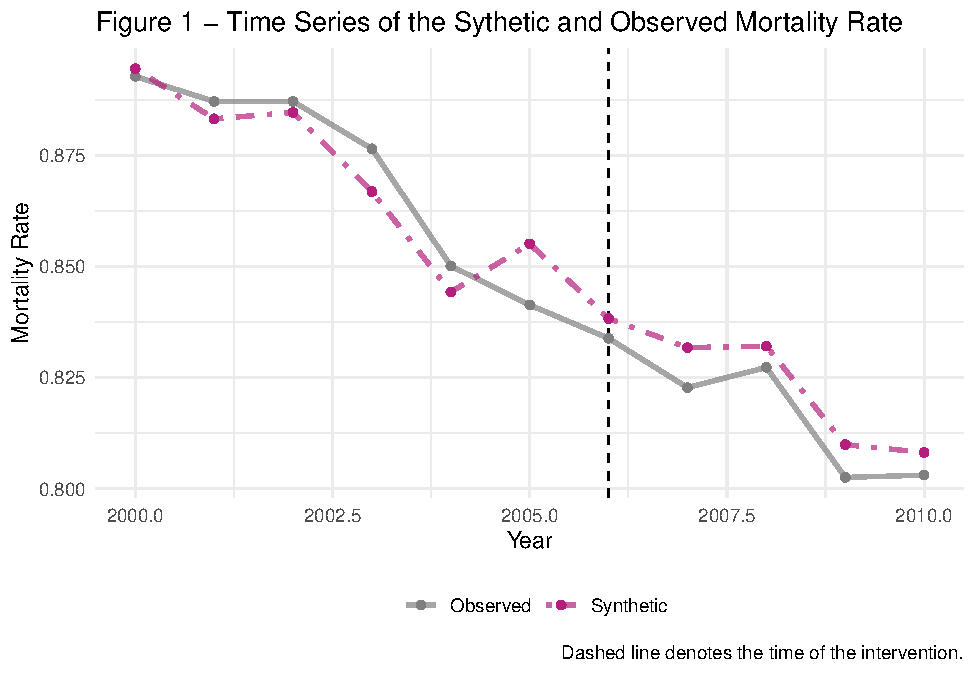
\includegraphics{report_files/figure-latex/figure1-1.pdf}

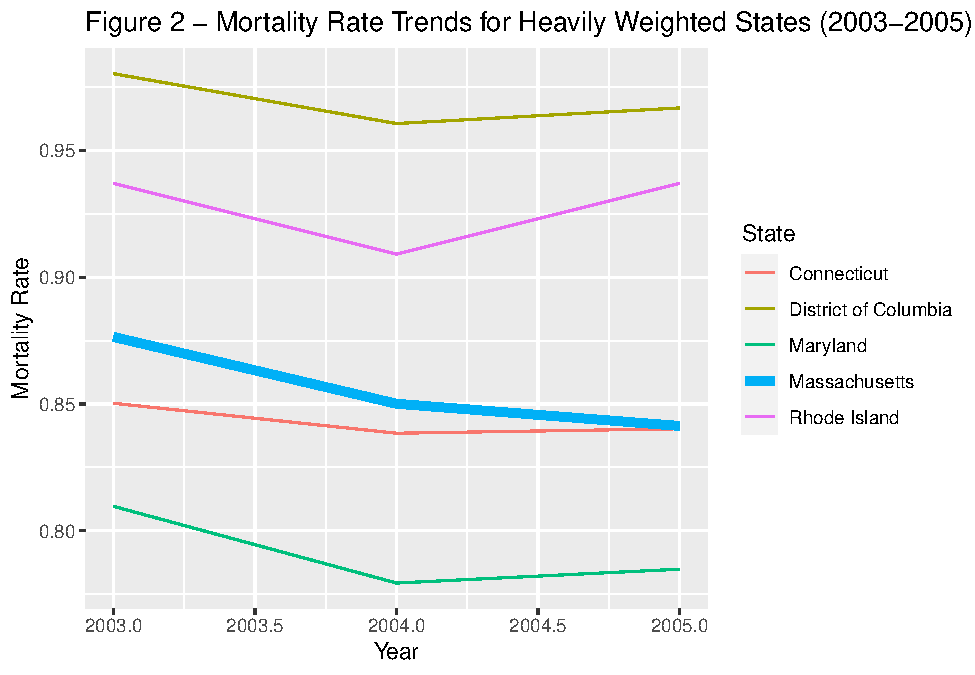
\includegraphics{report_files/figure-latex/figure2-1.pdf}

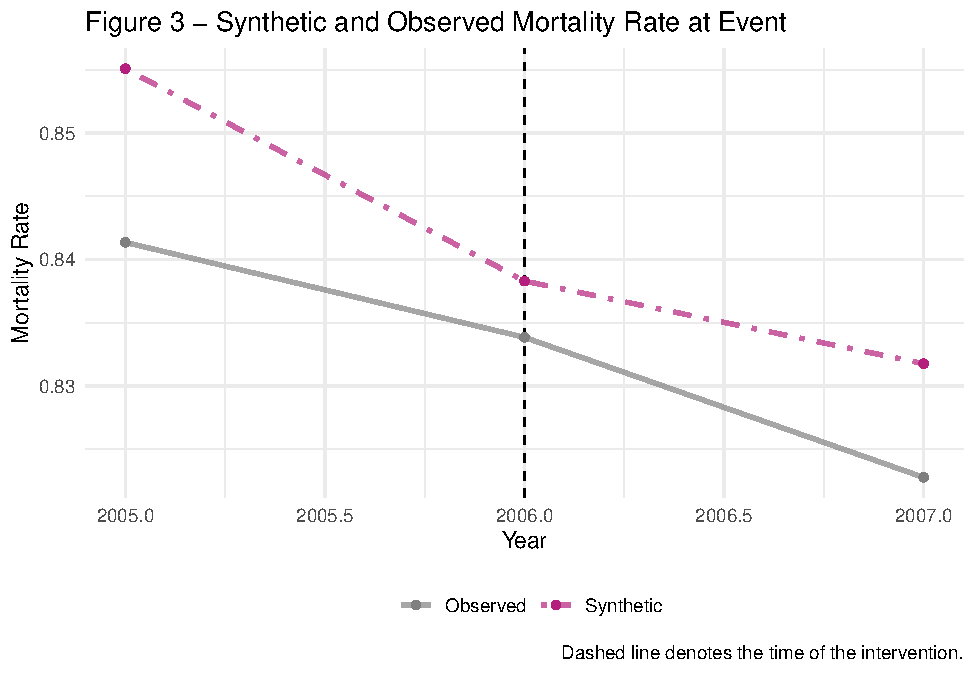
\includegraphics{report_files/figure-latex/figure3-1.pdf}

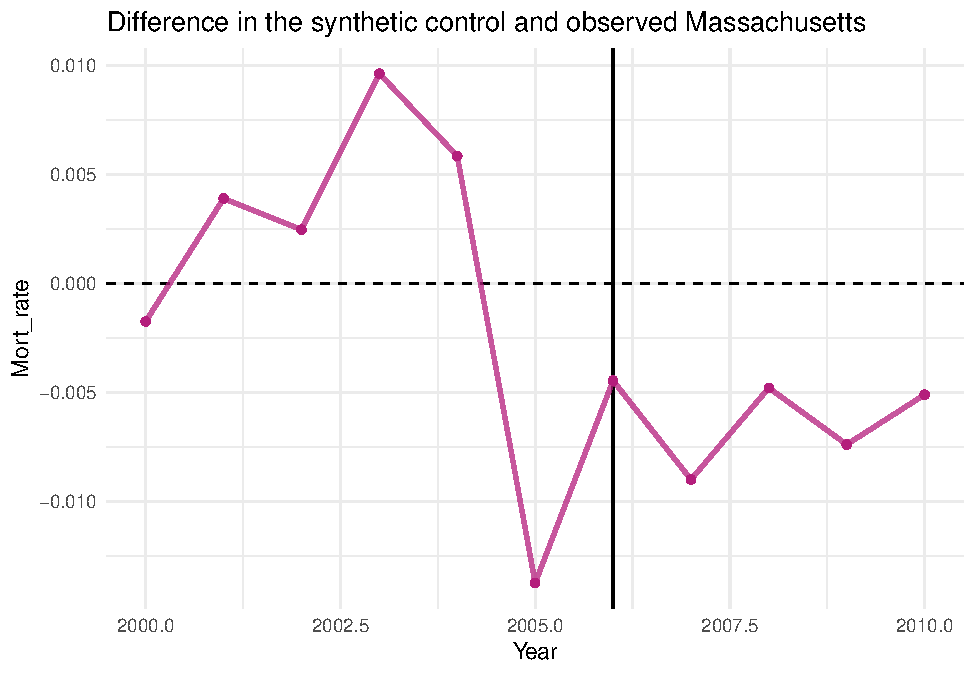
\includegraphics{report_files/figure-latex/table2g-1.pdf}

\hypertarget{conclusion}{%
\section{6. Conclusion}\label{conclusion}}

Low income households are experiencing subpar quality of healthcare as
well as the barriers to healthcare access as compared to their higher
income counterparts. It is a pressing issue that demands a carefully
crafted healthcare policy that can effectively promote better life
quality. The passage of Romneycare in 2006 in Massachusetts allows us to
estimate the effect of such health policy on mortality rates. States
such as Rhode Island, Maryland and Connecticut, are chosen with higher
weights to represent Massachusetts in the counterfactual world where it
was not treated. Our analysis reveals a significant decline in mortality
rates among nonelderly adults in Massachusetts. Although our results
only define average treatment on the treated, as opposed to the average
treatment effect for the entire population, since Massachusetts differs
from other states in many aspects such as its geography or demography.
Our research serves as a starting point for further analysis on the
treatment effects of healthcare policies.

\hypertarget{references}{%
\section{References}\label{references}}

Sommers, Benjamin D., Sharon K. Long, and Katherine Baicker. ``Changes
in Mortality after Massachusetts Health Care Reform.'' Annals of
Internal Medicine 160, no. 9 (May 6, 2014): 585.
\url{https://doi.org/10.7326/m13-2275}.

\end{document}
